\chapter{Mocap-Systeme}

Der Grossteil der Systeme kann in 3 Hauptklassen unterteilt werden. Magnetische, mechanische,
und optische Systeme. Es gibt es auch Hybridsysteme mit allen  
Kombinationen der Hauptklassensysteme. Es gibt viele Firmen, die eine Menge von solchen Geräten 
herstellen. Wir möchten nicht die einzelnen Produkte näher betrachten und beschreiben, sondern vielmehr die 
verschiedenen Systeme erklären.

\section{magnetische Systeme}

Bei den magnetischen Systemen arbeitet man mit Hall-Sensoren. Hall-Sensoren ermitteln ein magnetisches Feld aus, welches von einer Transmittereinheit gesendet wird. Bei diesem  Vorgang wird eine Ausgangsspannung bei den Hall-Sensoren erzeugt, welche dem Produkt aus Strom und magnetisches Feld entspricht. Über den ganzen Körper werden Hall-Sensoren verteilt (bevorzugt werden alle Gelenke). Die 
Sensoren übertragen ihre Daten zu einer Kontrolleinheit, die dann die Positionen im dreidimensionalen Raum berechnet.

\begin{figure}[htbp]
\centering
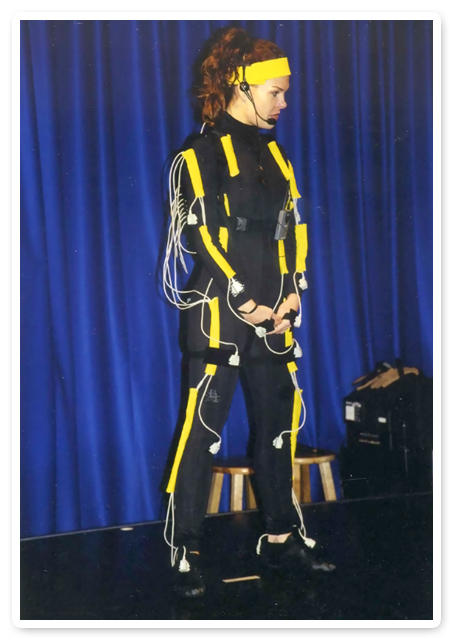
\includegraphics[scale=1]{include/magneticgirl.jpg}
\caption{Motion Capture Anzug eines magnetischen  Systems}
\end{figure}

Ein Nachteil ist, dass jeder Schauspieler mit Kabeln und Sensoren umzingelt ist, dadurch können sie sich nicht mehr ganz frei bewegen. Die Verkabelung ist notwendig, weil jeder Sensor eine Spannungsquelle benötigt. Die Akteuere tragen eine Batterie, meist als Rucksack oder versteckt im Anzug. All diese unhandlichen Konstruktionen fallen negativ auf die Bewegungsfreiheit der Akteure aus. \\
Ein weiterer Nachteil ist die Reichweite von magnetischen Systemen. Die Reichweite der Transmitter ist beschränkt und die Spielfläche muss mit einem Magnetfeld bestrahlt werden. Somit haben die Schauspieler meist eine bis zu Acht mal Acht Meter grosse Fläche zur Verfügung. \\
Der Vorteil bei den magnetischen Systemen ist, dass es hier keine Deckungsprobleme gibt wie bei den optischen Systemen. Bei einem optischen System
(siehe \ref{sec:optische_systeme} optische Systeme)
ist es schwieriger, alle Akteure Anhand von Punkten zu unterscheiden und einzelne Personen zu segmentieren. 
Jedoch können zwei Akteure die unmittelbar nebeneinander agieren, zum Beispiel bei einer Kampfszene bei der die Sensoren vom gegenüberliegenden Akteur gestört werden, das Ausgangssignal ebenso verfälschen. Es können auch andere elektrische Geräte oder Metall in der Umgebung das elektromagnetische Feld stören und somit zu einem schlechten Resultat führen. Der Vorteil ist, dass die Aufnahmen in Echtzeit stattfinden und verwendet werden können.

\section{Mechanische Systeme}

Anders als bei magnetischen Systeme benötigt man hier weder Sensoren noch eine Transmittereinheit. Bei mechanischen Systemen werden die Bewegungen direkt am Körper ausgelesen. Der Schauspieler trägt eine Art Aussenskelett mit jeweils Stangen für Ober- und Unterschenkel und für den Kopf und Rücken. Durch die Bewegungen der Stangen wird die Spannung über einem regelbaren Widerstand (Potentiometer) an den Gelenken verändert und ausgelesen. Diese analogen Spannungsänderungen werden in ein digitales Signal umgewandelt und von der Software interpretiert.
Mit Hilfe eines Gyroskop-Sensors (Kreisel) werden die Neigungen gemessen und somit lassen sich alle Körperbewegungen rekonstruieren. 

\subsubsection{Kalibrierung}
Die Kalibrierung ist hier Zeitaufwändig, da sie genau dem Schauspieler angepasst werden muss. Die Abstände zwischen den Gelenken muss genau erfasst werden, damit das Resultat höchstmöglich präzise ermittelt werden kann. Ein weiterer Grund dafür ist, dass der Schauspieler nicht an seiner Beweglichkeit limitiert sein soll und alle Bewegungen ausführen kann. \\
Diese Anpassung des Systems muss also für jeden einzelnen Schauspieler angepasst werden. Im Gegenteil zu den magnetischen und optischen Systemen, wo ganz am Anfang die Kameras justiert werden und gegebenenfalls nachkorrigiert werden müssen, kann hier eine Kalibrierung bis zu einer halben Stunde dauern. Wenn die Einstellungsdaten gespeichert wurden können sie innerhalb von 5 Minuten geladen werden und das System ist einsatzbereit.

\subsubsection{Vor- und Nachteile}
 Hier gibt es keine Probleme mehrere Personen miteinander aufzuzeichnen, da es keine Sensoren gibt die sich beeinflussen könnten wie bei magnetischen Systemen. Aber grundsätzlich ist man eingeschränkt in der Bewegungsfreiheit, wenn man an eine Kampfszene denkt oder Turneinlagen. Mit solchen Aussenskelette ist es nahezu unmöglich solche Szenen nach zuspielen. \\
 Dies ist auch der Grund, warum sich dieses System nicht durchgesetzt hat im Bereich Computerspiele, da man zu wenig Bewegungsfreiheit hat. Aber beispielsweise in der Rehabilitation von Patienten nach einem Unfall kann es durchaus Sinn machen ein solches System zu verwenden. Die Richtigkeit der Bewegungen kann nachvollzogen werden und dem Patienten helfen seinen Genesungsprozess zu optimieren.

\section{Optische Systeme}
\label{sec:optische_systeme}

Bei einem optischen System trägt der Schauspieler ebenso wie bei den anderen Systemen einen Ganzkörperanzug, der aber hier mit vielen reflektierenden Markern besetzt ist. Mit Hilfe von Kameras werden diese reflektierende Punkte (Markern) aufgenommen und am Rechner ausgewertet. Es gibt auch Systeme, welche mit Infrarot arbeiten (siehe \ref{sec:kinect} Kinect). \\
Die Marker werden an den wichtigsten Positionen des Körpers angebracht. Dies sind vor allem die Gelenke, weil sie alle Endpunkte der Körperteile darstellen, welche sich tatsächlich auch bewegen können. Hier gilt, je mehr Marker vorhanden sind desto genauer kann die Bewegung rekonstruiert werden. Typische Positionen für die Marker sind: Kopf, Nacken, Schulter, Ellenbogen, Handgelenke, Beckenknochen, Knie und Fussgelenke.

\begin{figure}[htbp]
\centering
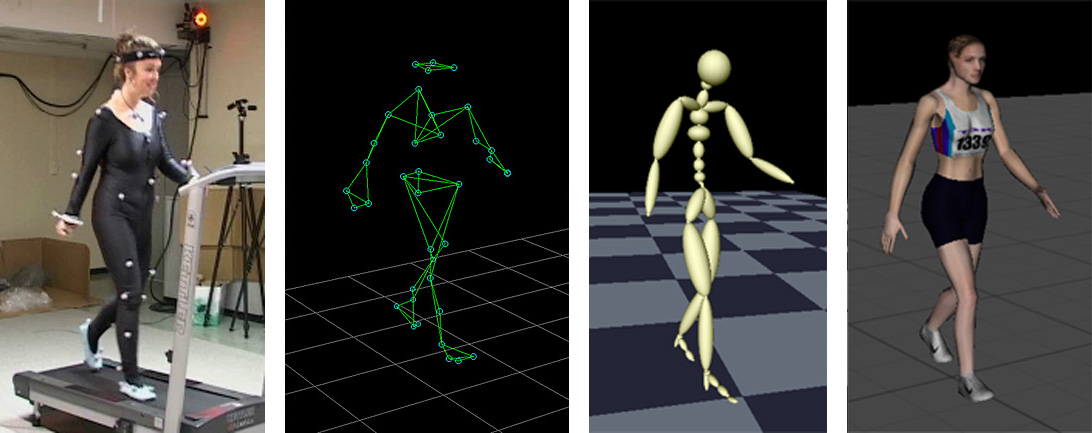
\includegraphics[scale=0.6]{include/opt_mocap.jpg}
\caption{(vlnr) Schauspielerin mit Markern ausgestattet auf einem Laufband; Kameraaufnahmen in ein Gitternetz-Model; Übertragung der Messwerte in ein simples 3D-Model; Animation einer Sprinterin}
\end{figure}

In dieser Abbildung erkannt man schön alle Schritte, welche notwendig sind um an ein gewünschtes Ziel zu gelangen. Die Statur der Animation muss einigermassen dem Ursprungsobjekt gleichen. Wenn wir annehmen folgende Frau im Bild wurde als Objekt in einem 3D-System dargestellt und als Model haben wir einen Gartenzwerg. Als Ziel verfolgen wir natürlich eine realistische Bewegungssequenz des Zwergen. \\
Nun haben wir aber das Problem, falls wir nur die Bewegungssequenzen der Beine in die Animation hinzufügen, der Zwerg zwar geht aber viel zu kleine Schritte macht oder wir verwenden die absolute Distanz, dies führt zu unnatürlichen bis zu unmöglichen Bewegungen des Zwerges. \\
Bisweilen gibt es keine Zauberformel, welche dieses Problem löst. Meist versuchen die Game-Designern die Animation selbst anzupassen mittels Keyframing und verwenden die Motion-Capture-Aufnahmen als Stütze und Ziel.

\subsubsection{Hero Pose}
Bevor überhaupt irgendwelche Aufnahmen getätigt werden können muss eine Kalibrierung stattfinden, damit das System die einzelnen Marker unterscheiden kann. Später folgt das System ununterbrochen den Markern und kann diese aufzeichnen. Hierfür steht der Akteur in die Mitte der Bühne und geht in die Heldenposition (die Haltung sieht aus wie ein grosses T). Damit soll gewährleistet sein, dass alle Marker sichtbar sind. Als ein modernes Beispiel dient hier Kinect.
 
\subsubsection{Kinect}
\label{sec:kinect}
Kinect ist eine Hardware zur Steuerung der Videospielkonsole Xbox 360. Kinect wurde von Microsoft mit der Zusammenarbeit von der Firma PrimeSense entwickelt. Spieler können statt mit einem Gamepad allein durch Körperbewegungen die Software bedienen. \\
Kinect ist mit einem Tiefensensor-Kamera, 3D-Mikrofon und Farbkamera ausgestattet. Die Tiefensensor-Kamera funktioniert folgendermassen: \\
Die Bühne wird mit Infrarotimpulse ausgeleuchtet und der Infrarot-Sensor in der Kamera misst für jeden Bildpunkt die Zeit, die das Licht bis zum Objekt und wieder zurück braucht. Die benötigte Zeit ist proportional zur Distanz. Das besondere an Kinect ist, dass die Spieler keine Marker benötigen. Durch die Tiefen-Wahrnehmung des Gerätes kann direkt ein 3D-Model der Umgebung im Computer  abgebildet werden. Somit wird der Prozess ``Übertragung der Marker-Aufnahmen in ein 3D Model'' übersprungen, stattdessen wird vom Computer ein eigenes Skelett berechnet, welches in die Szene passt.  
Kinect kann mit einer Auflösung von 1 cm in die Tiefe und 3mm auf der x und y-Achse genau bestimmen, wo die Objekte sich befinden. In der Tiefe ist es mit 3.5 Meter limitiert. \\

\begin{figure}[hbtp]
\centering
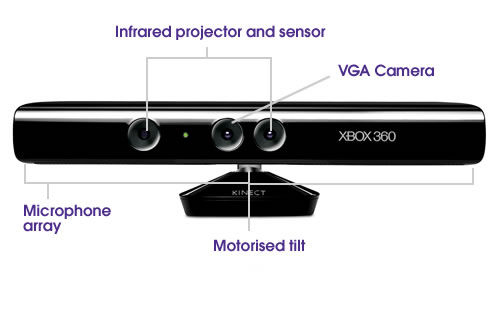
\includegraphics[scale=0.5]{include/kinect.jpg}
\caption{Kinect-Hardware}
\end{figure}

Auch ein Motor ist eingebaut, damit kann das Gerät geschwenkt und somit dem Spieler gefolgt werden.
Anhand von Kinect können wir erkennen, dass Motion Capturing unser Alltag schon längst bestimmt. Letztens wurde von Microsoft ein Software-Development-Kit vorgestellt um Hobby-Programmierer zu animieren an diesem Gerät zu arbeiten. Weiter wurde ein Open-Source-Treiber unter Windows und Linux freigegeben, welcher noch mehr Möglichkeiten hervorruft.

\subsubsection{Vor- und Nachteile}

Vorteile von optischen Systemen ist die sehr hohe Messgenauigkeit bzw. hohe Abtastrate, grosse Bewegungsfreiheit, man hat keine störende Einheiten am Anzug (nur kleine Licht-Reflektoren (Markern)) und die Möglichkeit mehrere interagierende Akteure gleichzeitig aufzuzeichnen. Das Arbeitsvolumen ist nur durch die Aufnahmefähigkeit der Kameras begrenzt. \\
Ein grosser Nachteil ist die fehlende Identifikation der Marker. Am Anfang bei der ``Hero Position'' ist es mühelos möglich alle Marker zu unterscheiden doch später bei Bewegungen, bei denen einige Marker abgedeckt sind, wird es schwierig diese zu finden. Hier muss meist von Hand nachgearbeitet werden. Oft werden verschiedenfarbige Marker eingesetzt um die Identifikation zu gewährleisten. Auch ist es so möglich ein vorübergehend abgedeckter Marker später anhand seiner Farbe wieder zu ``erkennen'' und aufzuzeichnen. \\
Bei völlig verdeckten Markern ist die Nachbearbeitung nicht zu vermeiden. 
